\documentclass[conference]{IEEEtran}
% \IEEEoverridecommandlockouts
% The preceding line is only needed to identify funding in the first footnote. If that is unneeded, please comment it out.
\usepackage{cite}
\usepackage{url}
\usepackage{amsmath,amssymb,amsfonts}
\usepackage{algorithmic}
\usepackage{tikz}
\usetikzlibrary{positioning}
\usepackage{graphicx}
% LaTeX Symbols: https://tug.ctan.org/info/symbols/comprehensive/symbols-a4.pdf
\usepackage{halloweenmath}
\usepackage{caption}
\captionsetup{justification=raggedright,singlelinecheck=false} % Align figure captions to the left
\usepackage{textcomp}
\usepackage{xcolor}
\def\BibTeX{{\rm B\kern-.05em{\sc i\kern-.025em b}\kern-.08em
    T\kern-.1667em\lower.7ex\hbox{E}\kern-.125emX}}
        
\begin{document}

\title{Memory corruption vulnerabilities: Modern safeguards and their shortcomings}

\author{\IEEEauthorblockN{Charles Zumbaugh}
\IEEEauthorblockA{\textit{Dept. of Computer Science} \\
\textit{Kansas State University}\\
Manhattan, Kansas \\
cazumbaugh@ksu.edu}
}

\maketitle

\begin{abstract}
Memory corruption vulnerabilities are a class of software security vulnerabilities that occur when a system's memory is altered in an unintended way. In many cases, the result of memory corruption is a program crash or unintended behavior; however, many of these bugs can be exploited by malicious actors to gain unauthorized access to the system. Despite the advent of memory-safe languages and considerable effort identifying and fixing the sources of these vulnerabilities in memory-unsafe languages, this class of vulnerability remains one of the most common attack vectors in cyber-systems. Most modern computers include both hardware and operating system features to prevent an attacker from successfully exploiting these bugs, but nevertheless, attackers can bypass many of these protections. This paper discusses common memory corruption vulnerabilities, several modern safeguards to protect cyber-systems, and strategies that can be used to circumvent them.
\end{abstract}

\begin{IEEEkeywords}
memory corruption, security, vulnerability, systems, malware
\end{IEEEkeywords}

\section{Introduction}
As computers have become more embedded in everyday life, the security of these systems has become a critical concern. Cyber attacks against government and non-government organizations has increased in recent years, particularly those targeting healthcare and large, multinational companies \cite{hammouchi2019digging}. As personal data is increasingly being collected and stored on servers, the scale of these breaches is also increasing. For example, a recent breach of Change Healthcare in 2025 exposed the personal data of more than 192 million individuals in the United States \cite{privacyrights2025}. The financial implications of security vulnerabilities are substantial, and IBM estimated the cost of a data breach in 2025 to be \$4.4 million \cite{ibm2025}.

Despite being recognized as a critical vulnerability over 30 years ago, and numerous approaches being developed to mitigate them, memory corruption vulnerabilities are still found in all types of software \cite{llorente2021neverending}. Indeed, the 2024 list of the top 25 most dangerous software vulnerabilities included buffer overflows and use-after free in the second and eighth positions, respectively \cite{cwe2024}. When exploited, these vulnerabilities can allow for arbitrary code execution, privilege escalation, and information leakage. 

In practice, a program is considered memory safe as long as a set of memory errors can never occur \cite{llorente2021neverending}, though rigorous, formal definitions have been presented in recent years \cite{azevedo2018meaning}. Memory corruption is due to the lack of memory safety in low-level languages such as C and C++, and while memory and type safe languages such as Java and Rust provide memory safety, the use of memory-unsafe languages is ubiquitous in systems programming. Additionally, mitigation techniques are not always used, even among modern operating systems. These techniques may require non-existent hardware support on older systems, have large performance costs, or require recompilation of critical components \cite{van2012memory}. 

\section{Overview of memory corruption vulnerabilities}
Memory corruption occurs when a system's memory is altered in an unintended way. These vulnerabilities are generally the result of subtle programming mistakes in low-level languages, where programmers must manually manage the memory throughout execution. Memory corruption will cause a crash or undefined behavior in many cases, but attackers can exploit memory errors to gain unauthorized access to the system by carefully modifying key regions of memory. While memory corruption vulnerabilities share some common characteristics as a class, their details differ and warrant discussion. 

\subsection{Buffer Overflow Vulnerabilities}
Buffer overflows are one of the most common and dangerous memory corruption vulnerabilities. A buffer overflow can occur when a program writes data to a memory buffer without checking the bounds. If the data is larger than the buffer, the program will continue to write into adjacent regions of memory. These adjacent regions commonly contain important information, such as return addresses, that can be modified by an attacker to allow for arbitrary code execution. 

\begin{figure*}[ht]
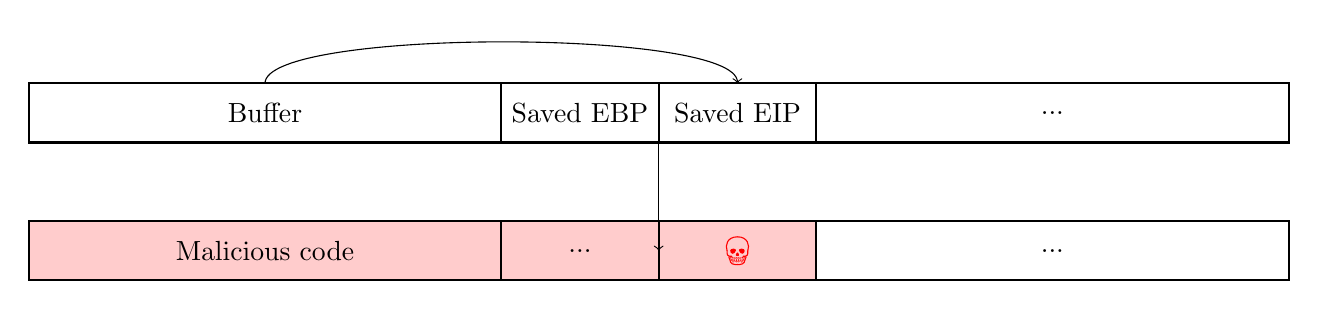
\begin{tikzpicture} [
	buffer/.style={rectangle, draw=black, thick, minimum height=0.75cm, minimum width=6cm, outer sep=0pt, inner sep=0pt},
	word/.style={rectangle, draw=black, thick, minimum height=0.75cm, minimum width=2cm, outer sep=0pt, inner sep=0pt}
]
% Memory cells
\node[buffer] (buffer1) {Buffer};
\node[word] (ebp1) [right=0cm of buffer1] {Saved EBP};
\node[word] (eip1) [right=0cm of ebp1] {Saved EIP};
\node[buffer] (rest1) [right=0cm of eip1] {...};

\node[buffer, fill=red!20] (buffer2) [below=1cm of buffer1] {Malicious code};
\node[word, fill=red!20] (ebp2) [right=0cm of buffer2] {...};
\node[word, fill=red!20] (eip2) [right=0cm of ebp2] {\color{red}$\bigskull$};
\node[buffer] (rest2) [right=0cm of eip2] {...};

% Arrows
\draw[->] (buffer1.north) .. controls +(up:7mm) and +(up:7mm) .. (eip1.north);
\draw[->] (eip1.west) -- (eip2.west);
\end{tikzpicture}
\caption{Example of a typical buffer overflow attack}
\end{figure*}

\subsection{Use After Free}


\subsection{Double Free}\label{AA}

\subsection{Units}
\begin{itemize}
\item Use either SI (MKS) or CGS as primary units. (SI units are encouraged.) English units may be used as secondary units (in parentheses). An exception would be the use of English units as identifiers in trade, such as ``3.5-inch disk drive''.
\item Avoid combining SI and CGS units, such as current in amperes and magnetic field in oersteds. This often leads to confusion because equations do not balance dimensionally. If you must use mixed units, clearly state the units for each quantity that you use in an equation.
\item Do not mix complete spellings and abbreviations of units: ``Wb/m\textsuperscript{2}'' or ``webers per square meter'', not ``webers/m\textsuperscript{2}''. Spell out units when they appear in text: ``. . . a few henries'', not ``. . . a few H''.
\item Use a zero before decimal points: ``0.25'', not ``.25''. Use ``cm\textsuperscript{3}'', not ``cc''.)
\end{itemize}

\subsection{Equations}
Number equations consecutively. To make your 
equations more compact, you may use the solidus (~/~), the exp function, or 
appropriate exponents. Italicize Roman symbols for quantities and variables, 
but not Greek symbols. Use a long dash rather than a hyphen for a minus 
sign. Punctuate equations with commas or periods when they are part of a 
sentence, as in:
\begin{equation}
a+b=\gamma\label{eq}
\end{equation}

Be sure that the 
symbols in your equation have been defined before or immediately following 
the equation. Use ``\eqref{eq}'', not ``Eq.~\eqref{eq}'' or ``equation \eqref{eq}'', except at 
the beginning of a sentence: ``Equation \eqref{eq} is . . .''

\subsection{\LaTeX-Specific Advice}

Please use ``soft'' (e.g., \verb|\eqref{Eq}|) cross references instead
of ``hard'' references (e.g., \verb|(1)|). That will make it possible
to combine sections, add equations, or change the order of figures or
citations without having to go through the file line by line.

Please don't use the \verb|{eqnarray}| equation environment. Use
\verb|{align}| or \verb|{IEEEeqnarray}| instead. The \verb|{eqnarray}|
environment leaves unsightly spaces around relation symbols.

Please note that the \verb|{subequations}| environment in {\LaTeX}
will increment the main equation counter even when there are no
equation numbers displayed. If you forget that, you might write an
article in which the equation numbers skip from (17) to (20), causing
the copy editors to wonder if you've discovered a new method of
counting.

{\BibTeX} does not work by magic. It doesn't get the bibliographic
data from thin air but from .bib files. If you use {\BibTeX} to produce a
bibliography you must send the .bib files. 

{\LaTeX} can't read your mind. If you assign the same label to a
subsubsection and a table, you might find that Table I has been cross
referenced as Table IV-B3. 

{\LaTeX} does not have precognitive abilities. If you put a
\verb|\label| command before the command that updates the counter it's
supposed to be using, the label will pick up the last counter to be
cross referenced instead. In particular, a \verb|\label| command
should not go before the caption of a figure or a table.

Do not use \verb|\nonumber| inside the \verb|{array}| environment. It
will not stop equation numbers inside \verb|{array}| (there won't be
any anyway) and it might stop a wanted equation number in the
surrounding equation.

\subsection{Some Common Mistakes}\label{SCM}
\begin{itemize}
\item The word ``data'' is plural, not singular.
\item The subscript for the permeability of vacuum $\mu_{0}$, and other common scientific constants, is zero with subscript formatting, not a lowercase letter ``o''.
\item In American English, commas, semicolons, periods, question and exclamation marks are located within quotation marks only when a complete thought or name is cited, such as a title or full quotation. When quotation marks are used, instead of a bold or italic typeface, to highlight a word or phrase, punctuation should appear outside of the quotation marks. A parenthetical phrase or statement at the end of a sentence is punctuated outside of the closing parenthesis (like this). (A parenthetical sentence is punctuated within the parentheses.)
\item A graph within a graph is an ``inset'', not an ``insert''. The word alternatively is preferred to the word ``alternately'' (unless you really mean something that alternates).
\item Do not use the word ``essentially'' to mean ``approximately'' or ``effectively''.
\item In your paper title, if the words ``that uses'' can accurately replace the word ``using'', capitalize the ``u''; if not, keep using lower-cased.
\item Be aware of the different meanings of the homophones ``affect'' and ``effect'', ``complement'' and ``compliment'', ``discreet'' and ``discrete'', ``principal'' and ``principle''.
\item Do not confuse ``imply'' and ``infer''.
\item The prefix ``non'' is not a word; it should be joined to the word it modifies, usually without a hyphen.
\item There is no period after the ``et'' in the Latin abbreviation ``et al.''.
\item The abbreviation ``i.e.'' means ``that is'', and the abbreviation ``e.g.'' means ``for example''.
\end{itemize}
An excellent style manual for science writers is.

\subsection{Authors and Affiliations}
\textbf{The class file is designed for, but not limited to, six authors.} A 
minimum of one author is required for all conference articles. Author names 
should be listed starting from left to right and then moving down to the 
next line. This is the author sequence that will be used in future citations 
and by indexing services. Names should not be listed in columns nor group by 
affiliation. Please keep your affiliations as succinct as possible (for 
example, do not differentiate among departments of the same organization).

\subsection{Identify the Headings}
Headings, or heads, are organizational devices that guide the reader through 
your paper. There are two types: component heads and text heads.

Component heads identify the different components of your paper and are not 
topically subordinate to each other. Examples include Acknowledgments and 
References and, for these, the correct style to use is ``Heading 5''. Use 
``figure caption'' for your Figure captions, and ``table head'' for your 
table title. Run-in heads, such as ``Abstract'', will require you to apply a 
style (in this case, italic) in addition to the style provided by the drop 
down menu to differentiate the head from the text.

Text heads organize the topics on a relational, hierarchical basis. For 
example, the paper title is the primary text head because all subsequent 
material relates and elaborates on this one topic. If there are two or more 
sub-topics, the next level head (uppercase Roman numerals) should be used 
and, conversely, if there are not at least two sub-topics, then no subheads 
should be introduced.

\subsection{Figures and Tables}
\paragraph{Positioning Figures and Tables} Place figures and tables at the top and 
bottom of columns. Avoid placing them in the middle of columns. Large 
figures and tables may span across both columns. Figure captions should be 
below the figures; table heads should appear above the tables. Insert 
figures and tables after they are cited in the text. Use the abbreviation 
``Fig.~\ref{fig}'', even at the beginning of a sentence.

\begin{table}[htbp]
\caption{Table Type Styles}
\begin{center}
\begin{tabular}{|c|c|c|c|}
\hline
\textbf{Table}&\multicolumn{3}{|c|}{\textbf{Table Column Head}} \\
\cline{2-4} 
\textbf{Head} & \textbf{\textit{Table column subhead}}& \textbf{\textit{Subhead}}& \textbf{\textit{Subhead}} \\
\hline
copy& More table copy$^{\mathrm{a}}$& &  \\
\hline
\multicolumn{4}{l}{$^{\mathrm{a}}$Sample of a Table footnote.}
\end{tabular}
\label{tab1}
\end{center}
\end{table}

\begin{figure}[htbp]
\centerline{\includegraphics{fig1.png}}
\caption{Example of a figure caption.}
\label{fig}
\end{figure}

Figure Labels: Use 8 point Times New Roman for Figure labels. Use words 
rather than symbols or abbreviations when writing Figure axis labels to 
avoid confusing the reader. As an example, write the quantity 
``Magnetization'', or ``Magnetization, M'', not just ``M''. If including 
units in the label, present them within parentheses. Do not label axes only 
with units. In the example, write ``Magnetization (A/m)'' or ``Magnetization 
\{A[m(1)]\}'', not just ``A/m''. Do not label axes with a ratio of 
quantities and units. For example, write ``Temperature (K)'', not 
``Temperature/K''.

\section*{Acknowledgment}

The preferred spelling of the word ``acknowledgment'' in America is without 
an ``e'' after the ``g''. Avoid the stilted expression ``one of us (R. B. 
G.) thanks $\ldots$''. Instead, try ``R. B. G. thanks$\ldots$''. Put sponsor 
acknowledgments in the unnumbered footnote on the first page.

\section*{References}
tnotes in the 
abstract or reference list. Use letters for table footnotes.


\bibliographystyle{IEEEtran}
\bibliography{references}    

\vspace{12pt}
\color{red}
IEEE conference templates contain guidance text for composing and formatting conference papers. Please ensure that all template text is removed from your conference paper prior to submission to the conference. Failure to remove the template text from your paper may result in your paper not being published.

\end{document}
